\documentclass{article}

\usepackage[utf8]{inputenc}
\usepackage{graphicx}
\usepackage[export]{adjustbox}
\usepackage[T1]{fontenc}
\usepackage{hyperref}
\hypersetup{
colorlinks=true,
linkcolor=blue,
filecolor=magenta,
urlcolor=cyan,
}

\urlstyle{same}

% Path relative to the main .tex file.
\graphicspath{ {./images/} }

\title{Scalavelli project}

\date{14 Agosto - 15 Settembre 2020}

\author{
Cavalluzzo M.
\and
Giorgetti L.
\and
Pagnini L.
\and
Tentoni D.
}

\begin{document}
  \pagenumbering{gobble} % no numbers.
  \maketitle
  \newpage
  \pagenumbering{arabic} % start counting numbers.

  \begin{center}
    Progetto scritto in Scala per giocare al celebre gioco Machiavelli sul proprio computer e sfidare altri giocatori.
  \end{center}

  \tableofcontents

  \newpage


  \section{Processo di sviluppo}\label{sec:processo-di-sviluppo}
  \subsection{Metodologia}
Sin da subito abbiamo deciso di adottare una metodologia di sviluppo \textit{Agile-Scrum}, seppur non scegliendo un vero e proprio Scrum Master.
Chi più e chi meno, a seconda dei vari sprint, ognuno ha avuto l'occasione e il modo di ricoprire tale ruolo.
In questo modo tutti hanno potuto dare il loro contributo per la riuscita del progetto, coordinando il team con l'aiuto degli strumenti a disposizione.
In accordo con tale metodologia, il lavoro è stato suddiviso in \textit{Sprint}, della durata media di una settimana e mezzo.
Allo scadere del tempo si sarebbe dovuti arrivare a sviluppare un numero minimo di funzionalità dell'applicativo.
I meeting sono stati frequenti all'inizio e ne sono stati svolti alcuni saltuariamente all'interno di ogni sprint.
Questo perché, alternandosi con un periodo di lavoro autonomo, abbiamo ritenuto necessario e producente confrontarsi anche durante gli sprint su scelte sintattiche e pattern di sviluppo tra tutti i membri del team, in modo da condividere conoscenze ed entusiasmo.
\subsection{Strumenti adottati}
\subsubsection{VCS}
Si è deciso di utilizzare \textit{Git} per effettuare il versioning del codice durante lo sviluppo attraverso la piattaforma \textit{GitHub}.
L’utilizzo che ne abbiamo fatto è descritto nella figura 1: il branch di default è sempre il \textit{master}, al quale \textit{dev} è sempre allineato.
Nel caso in cui debbano essere prodotti degli hotfix, essi vengono svolti su un branch che parte dal \textit{master} e vi ritorna subito, senza passare da \textit{dev}.
\begin{figure}
    \centering
    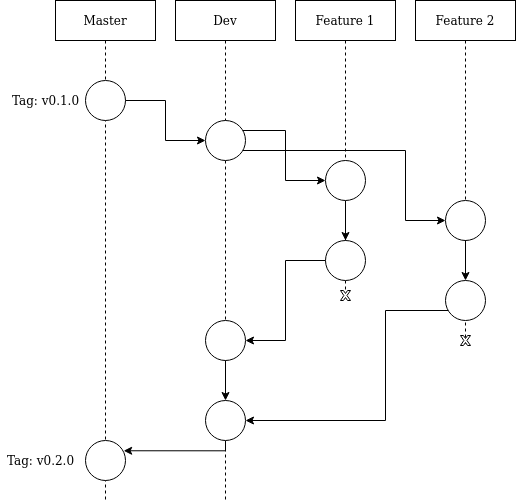
\includegraphics[scale=0.4]{git-workflow-1-1}
    \caption{GitFlow}
\end{figure}
Ogni volta che si implementava una nuova funzionalità o si risolveva una fix, veniva creato una branch a parte.
Successivamente, a lavoro ultimato, veniva una creata pull request per mergiare sul branch \textit{dev}.
Ogni pull request su \textit{dev} deve essere approvata almeno da un altro membro del gruppo.
Per mergiare invece un insieme di funzionalità sviluppate e testate dal branch \textit{dev} al \textit{master}, deve sempre essere aperta una pull request, che deve essere approvata da tutti i membri del gruppo.
Questo per essere certi che tutti i membri del gruppo siano consapevoli del lavoro svolto da tutti gli altri.

\subsubsection{Build Automation}
Si è deciso di usare \textit{SBT}, dato che durante il corso lo si é sempre preferito rispetto al 'cugino' \textit{Gradle} per lo svolgimento degli elaborati, nonostante il fatto che alcuni componenti del gruppo lo utilizzino in ambito aziendale.

\subsubsection{Continuous Integration}
Si è deciso di usare \textit{Travis CI}.
Consisteva nell'unica soluzione freeware che i componenti del gruppo abbiano mai usato, introdotta proprio in questo corso.
Tuttavia, è stato necessario approfondire l'argomento tramite studio autonomo, dato che ciò che si era appreso a lezione é stato ritenuto insufficiente per la buona riuscita del progetto per come è stato pensato.
Ad esso é stata adattata l'esecuzione dei test necessari per verificare la correttezza del lavoro svolto e poter poi effettuare dei rilasci senza regressioni.
Tramite lo stesso servizio é stata effettuata la \textit{Continuous Delivery}, rilasciando dei pacchetti compilati su \textit{Github Releases}.

\subsubsection{Bacheca}
Per avere una visione sull’andamento generale del progetto e sulle specifiche feature da svolgere o completate, abbiamo utilizzato \textit{Trello}.
\newline
Si sono realizzate delle etichette personalizzate (figura 2) da associare alle feature da implementare per una migliore organizzazione per ogni membro del team. Inoltre si sono create delle colonne (figura 3) in cui raggruppare le feature a seconda del suo stato di sviluppo.
Alcune di queste sono:
\begin{itemize}
    \item \textit{To Do}: contiene le card associate alle features da sviluppare;
    \item \textit{Done}: contiene le card associate alle features sviluppate;
    \item \textit{Bug}: contiene le card associate alle features che presentano bug da ‘fixare’;
    \item \textit{Sprint}: contiene le card che riassumono le features da svolgere per ogni sprint.
\end{itemize}
\begin{figure}
    \centering
    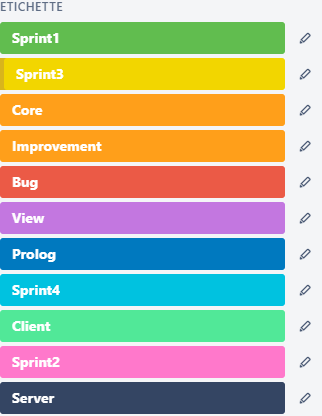
\includegraphics[width=5cm]{etichetteTrello}
    \caption{Etichette personalizzate}
\end{figure}
\begin{figure}
    \centering
    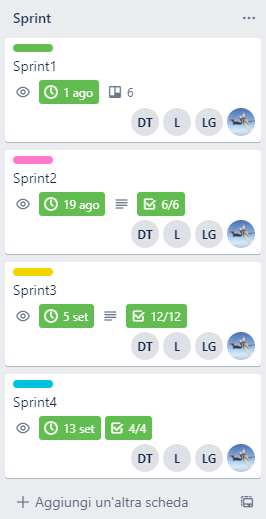
\includegraphics[width=5cm]{SprintTrello}
    \caption{Lista degli sprint}
\end{figure}
La bacheca è possibile consultarla direttamente cliccando il link:   \href{https://trello.com/b/Nk4j3Kuf/pps}{Trello}.
\subsubsection{Test}
Durante il progetto si è data importanza anche allo sviluppo dei test.
In particolare ogni membro del team, ha testato tutte le features da lui sviluppate creandone ad-hoc utilizzando l'approccio più consono.
Ogni sviluppatore prima di poter eseguire una pull request della propria features, doveva controllare che i test eseguiti passassero non solo in locale ma anche sul server di CI.
Lo sviluppo dei test è stato di aiuto soprattutto negli Sprint 3 e 4 poiché ci hanno permesso di individuare e di risolvere i bug più velocemente.
\newpage


  \section{Requisiti}\label{sec:requisiti}
  \subsection{Business}
Il progetto Scalavelli vuole ricreare l’esperienza del celebre gioco di carte Machiavelli (Ramino Machiavellico) in modalità multiplayer, tra giocatori differenti collocati sulla stessa macchina o nella stessa LAN. Ogni giocatore deve potersi identificare con un proprio username e connettersi ad una lobby.
Essa deve poter contenere da 2 a 6 giocatori.
Raggiunto il numero necessario di essi si potrà partecipare ad una partita.
Vi è anche la possibilità di scegliere di giocare specificatamente con i propri amici inserendo il codice identificativo per una partita privata.

\subsection{Utente}
L’utente medio utilizzatore potrà interagire solamente con il client (come descritto in seguito).
Le operazioni in fase di creazione della partita sono:
\begin{itemize}
    \item Specificare il proprio username (per potersi registrare nel server) e il numero di giocatori di una partita pubblica;
    \item Specificare il proprio username, il numero di giocatori e generare o specificare un codice per una partita privata;
    \item Creare una lobby privata;
    \item Connettersi ad una lobby e attendere il raggiungimento del numero di giocatori.
\end{itemize}
Dopo aver generato una partita ed esservi entrato, in una nuova schermata il giocatore potrà:
\begin{itemize}
    \item Vedere sullo schermo le combinazioni che ci sono attualmente sul tavolo da gioco, le carte che ha in mano, il nome degli altri giocatori e il numero di carte nelle loro mani;
    \item Solamente nel proprio turno, eseguire le seguenti azioni:
    \begin{itemize}
        \item Giocare una combinazione: si possono mettere sul tavolo da giocare una sequenza di carte che compongono una combinazione tra un tris, un poker oppure una scala.
        Se la combinazione è valida, allora vengono tolte le carte che si vuole giocare dalla mano e vengono messe sul tavolo;
        \item Aggiungere carte ad una combinazione sul tavolo già esistente: si possono scegliere delle carte dalla propria mano, che non necessariamente compongono una combinazione valida e mettere assieme alle carte che compongono un’altra combinazione, a patto che venga sempre rispettata la validità della combinazione;
        \item Prendere delle carte dal tavolo: si possono scegliere delle carte che appartengono ad una combinazione presente sul tavolo da gioco e metterle nella propria mano.
        \item Passare il turno al giocatore successivo: dopo che viene eseguita questa azione, il turno viene passato al giocatore successivo.
        Il giocatore che ha eseguito questa azione non ne può effettuare nessun’altra fino a che non riprende il proprio turno dall’azione del giocatore precedente nell’ordine.
        Nel caso in cui il giocatore di turno:
        \begin{itemize}
            \item non avesse eseguito nessuna mossa;
            \item avesse in mano delle carte che ha preso dal tavolo da gioco senza averle rigiocate;
            \item se non si trovasse con meno carte in mano rispetto a quando ha iniziato il turno;
            \item se scade il tempo a disposizione;
        \end{itemize}
        allora è costretto a pescare una carta dal mazzo principale.
    \end{itemize}
\end{itemize}

\subsection{Funzionali}
\begin{center}
    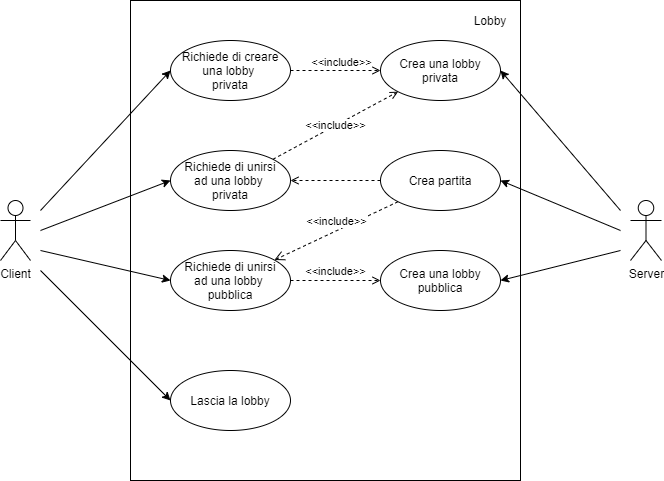
\includegraphics[scale=0.4]{casiDUso_Lobby}
\end{center}
\space
\hspace{4cm}Esempio di gestione lobby
\subsubsection{Connessione al server e creazione della lobby}
Il sistema dovrà:
\begin{itemize}
    \item Permettere al client di connettersi a internet;
    \item Una volta connessi al server permettersi di unirsi ad una lobby attraverso il proprio username;
    \item Assicurarsi che il server mantenga sempre attiva la connessione con il client, per poter inviare e ricevere messaggi inerenti alla partita;
    \item Assicurarsi che qualora venga raggiunto il numero di giocatori necessario, il server dovrà subito far partire la partita tra i giocatori;
    \item Nel caso in cui un giocatore venga disconnesso dalla partita, sia una disconnessione volontaria o un problema dell’infrastruttura di rete, terminare la partita per tutti, venendo visto come un abbandono;
    \item Al termine di una partita permetterne di iniziarne una nuova.
\end{itemize}
\begin{center}
    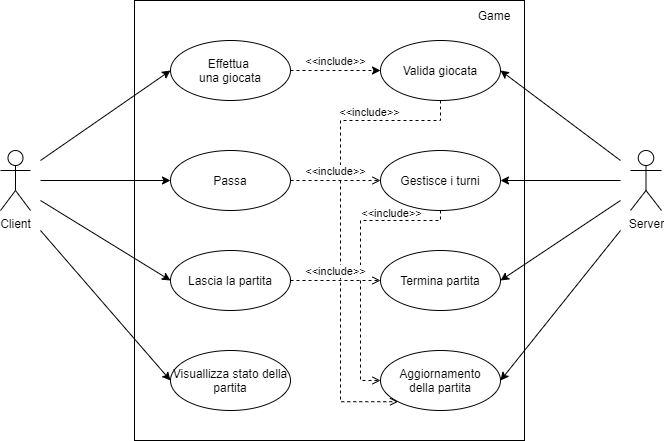
\includegraphics[scale=0.4]{casiDUso_Game}
\end{center}
\hspace{4cm}Esempio di gestione partita
\subsubsection{Gioco}
All’inizio della partita vengono mischiati due mazzi da 52 carte ognuno e distribuite 13 carte ad ogni giocatore.
Nel proprio turno si ha un tempo massimo di 2 minuti per svolgere le proprie mosse.
Una volta scaduto, tutte le mosse effettuate vengono annullate, si pesca una carta e si passa il turno al giocatore successivo.
In ogni momento devono sempre essere visibili:
\begin{itemize}
    \item le proprie carte in mano;
    \item il tavolo da gioco con le varie combinazioni;
    \item gli altri giocatori, con i loro nomi e il numero di carte nelle loro mani.
\end{itemize}

\subsection{Non Funzionali}

\subsubsection{Scalabilità}
Il server deve essere in grado di supportare un numero indefinito di utenti nell’insieme di tutte le partite.
Nel caso in cui non ci siano abbastanza giocatori in coda per iniziare una partita, allora questi devono essere lasciati in attesa dall’arrivo di altri giocatori che vogliano giocare anche loro.
Il sistema non consente l’accesso ad altri utenti per una partita specifica quando questa ha raggiunto il numero di partecipanti richiesto.

\subsubsection{Modularità}
Il progetto è stato pensato in modo tale da dover effettuare meno modifiche possibili al client nel caso in cui debba essere cambiato il server e viceversa.
Nello specifico: se il server deve subire un aggiornamento, esso dovrebbe essere spento e poi riacceso.
Gli utenti finali non devono eseguire nessuna operazione sui loro client, o almeno l’aggiornamento deve essere mantenuto il più piccolo possibile.
Viceversa, nel caso di aggiornamento dei client, non dovrebbe essere necessario né riavviare il server, né aggiornare nessuna sua parte.
Tutto il software deve riuscire a funzionare anche cambiando l’implementazione interna del modulo del “core” (regole e logica di gioco) a patto di non impattare sull’interfaccia dello stesso.

\subsubsection{Usabilità}
Il sistema deve fornire agli utenti un'interfaccia chiara, semplice, ben organizzata in modo da poter utilizzare al meglio tutte le sue funzionalità messe a disposizione e visualizzate.

\subsubsection{Reattività}
Il sistema deve poter consentire di giocare una partita senza ritardi e/o blocchi temporali dati dall’esecuzione degli algoritmi di validazione e controllo e dai protocolli di comunicazione.

\subsubsection{Sicurezza}
Il sistema deve aver sempre la possibilità di controllare lo stato attuale del gioco in modo da impedire che alcuni giocatori possano "iniettarne" uno non veritiero nella partita attuale.
Per questo ad ogni fine turno deve essere validato da parte del server in modo che un client malevolo non possa rovinare l’esperienza di gioco agli altri giocatori.

\subsection{Implementativi}
Di seguito vengono descritti i vincoli che abbiamo cercato di rispettare per l’intero sviluppo del progetto:
\begin{itemize}
    \item Mantenere un approccio il più funzionale possibile;
    \item Mantenere, in tutti i casi in cui era possibile, una stato immutabile nei vari componenti del sistema.
\end{itemize}
Principali tecnologie e modelli utilizzati sono:
\begin{itemize}
    \item Scala: Il sistema deve essere prevalentemente sviluppato in scala.
    \item ScalaFX: Il sistema deve disporre di un’interfaccia grafica per poter interagire con il gioco e il server.
    \item Prolog: Utilizzo del prolog per implementare l’ordinamento delle carte (per seme e valore), le entità del gioco e la validazione della correttezza delle combinazioni di carte.
    \item Akka: Utilizzo di varie componenti per implementare un server e un client che comunichino, secondo il paradigma di programmazione ad attori, per mezzo di messaggi asincroni.
    \item TDD (Test Driven Development): Ci siamo ispirati a questa tecnica di sviluppo per scrivere un codice più efficiente, efficace e il più possibile esente da problemi.
\end{itemize}
\newpage


  \section{Design Architetturale}\label{sec:design-architetturale}
  Per gestire l'ambito multiplayer è stata realizzata un’architettura \textit{Client}-\textit{Server}.
Ogni giocatore è rappresentato dal \textit{Client} mente un unico \textit{Server} si occupa di gestire le varie connessioni con i \textit{Client} e lo stato delle partite.

\subsection[Architettura]{Architettura}

\subsubsection{Core}
E’ stato poi realizzato, in maniera indipendente dalle altre componenti, un modulo di gioco che si occupa della sola gestione del gioco stesso, ovvero Machiavelli.
Esso definisce unicamente le entità base e le regole che lo caratterizzano.
Esso può essere considerato come fosse un libreria esterna che non mantiene alcun stato relativo al gioco in corso, ma espone solamente delle API che possono essere utilizzate da chiunque.
Nel nostro caso sia dal Server ma anche dal \textit{Client}: dal primo per gestire lo stato globale della partita ed aggiornarla in risposta alle mosse dei vari giocatori, dal secondo per gestire internamente la fase del turno, validando le mosse effettuate, in cui l’utente può effettuare una quantità di mosse a piacimento interfacciandosi col core, per poi inviare al \textit{Server} il riepilogo delle azioni effettuate a fine turno.
Questo componente è stato realizzato integrando i linguaggi \textit{Scala-Prolog}.

\subsubsection{Server}
Il \textit{Server} è la componente principale del sistema, si occupa di gestire le connessioni con i \textit{Client} durante la fase di matchmaking, di creare le varie partite di gioco e di mantenere lo stato.
E’ diviso internamente in più componenti ed è costituito da 2 componenti principali:
\begin{itemize}
    \item \textit{LobbyManagerActor}: si occupa della gestione della lobby.
    È a lui che i Client chiedendo di giocare.
    Una volta raggiunte le condizioni necessarie per avviare una partita, genera un GameMatchManager che si occuperà da quel momento in poi della gestione del gioco.
    \item \textit{GameMatchManagerActor}: si occupa di gestire una partita in corso.
    In fase di runtime ne saranno presenti molteplici attivi contemporaneamente, uno per ogni partita.
    Mantiene lo stato della partita corrente e di gestire i turni di gioco, ricevendo le azioni da ogni utente e comunicando a tutti gli altri ogni aggiornamento avvenuto.
\end{itemize}

\subsubsection{Client - MVC}
É utilizzato dall’utente per poter cercare una partita secondo le proprie preferenze e per giocare la stessa.
Internamente realizzato seguendo il pattern MVC, è poi ulteriormente diviso in due macro parti che rispecchiano all’incirca quello già visto sul \textit{Server}:
\begin{itemize}
    \item Una di gestione della fase iniziale di gioco, ovvero la lobby, utilizzata per poter ricercare la partita desiderata;
    \item Una di gestione del gioco stesso, utilizzata nel momento in cui la partita è in esecuzione, con cui l’utente può effettuare mosse durante il proprio turno, comunicarle al server e ricevere gli aggiornamenti conseguenti alle azioni effettuate dagli altri giocatori.
\end{itemize}

\subsubsection{Comunicazione client-server}
Tra il \textit{Client} e il \textit{Server} si è scelto di utilizzare un modello di comunicazione a scambio di messaggi, realizzata grazie all’utilizzo del framework \textit{Akka}.
Questa scelta ha permesso di gestire ad alto livello le comunicazioni tra le componenti senza preoccuparsi dei dettagli implementativi della comunicazione stessa.

\subsubsection[Flussi di interazione]{Flusso di interazione client server}
%todo: aggiungere grafico d'interazione.
Il grafico seguente riassume gli aspetti visti in precedenza nei paragrafi relativi alla parte \textit{Client} e \textit{Server}, mostrando come la parte del flusso di gioco del turno del giocatore venga gestito completamente in locale, mentre il \textit{Server} viene contattato solo al suo termine per validare le mosse effettuate dal giocatore e inviare lo stato aggiornato a tutti gli altri.
Questa scelta è stata fatta per garantire ottime prestazioni durante il gioco.
La fase del turno è infatti quella caratterizzata dalla frequenza più elevata di interazioni utente (riposizionamento carte, ordinamento della carte in mano, annullamento delle mosse precedenti ecc..), tutte operazioni non di rilevanza per gli altri giocatori connessi, a cui interessa più che altro lo stato finale del turno dell’avversario.
Il sistema è stato comunque modellato in maniera tale da prevedere modifiche future anche sotto questo aspetto, in maniera da spostare tutto lato server o lato client a seconda delle esigenza (ad esempio in una modalità singolo giocatore vs AI).

\newpage

  \section{Design di Dettaglio}\label{sec:design-di-dettaglio}
  \subsection{Organizzazione del codice}
La suddivisione del codice rispecchia fortemente il design architetturale generale descritto in precedenza.
\begin{center}
    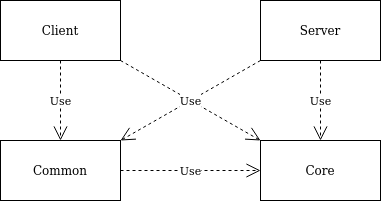
\includegraphics[scale=0.5]{moduli}
\end{center}
Sono stati realizzati 4 moduli:
\begin{itemize}
    \item Core: comprende tutte le entità necessarie alla realizzazione del gioco e le regole per poter portare avanti una partita, è l’unico tra i moduli totalmente indipendente dagli altri;
    \item Common: codice comune alle parti di client e server, per la maggior parte definisce i messaggi utilizzati per lo scambio di informazioni;
    \item Client: contenente tutto ciò che concerne il client, interfaccia utente, parte di comunicazione con il server e di aggiornamento dello stato della partita;
    \item Server: contenente tutta la parte di gestione delle lobby e delle partite in corso.
\end{itemize}
\subsection{Core}
Il core modella al suo interno tutte le entità del gioco Machiavelli reale, come le carte, il mazzo, il tavolo da gioco e la \textit{GameInterface}, cioè un insieme di funzioni che gli altri moduli del progetto devono usare per poter interagire con le entità. Tali funzioni infatti modellano tutte le azioni che un giocatore può svolgere nel gioco reale.
\subsubsection{Entità}
\begin{center}
    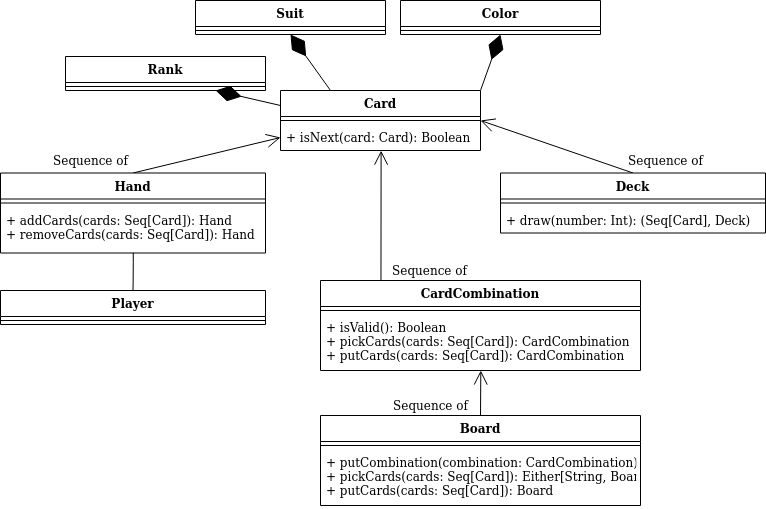
\includegraphics[width=\textwidth]{classi-Page-1}
\end{center}
Le entità di gioco sono:
\begin{itemize}
    \item la card, corredata da tre case class: un rank (valore nominale), un seme e un colore.
    All’interno del Rank si sono definiti tutti i possibili valori che una carta può assumere (da 1 a 13). Inoltre è stato modellato anche il caso del rank asso come 14-esimo valore, chiamato \textit{overflowAce}, per poterne effettuare la validazione qualora si trovasse dopo il Re (13-esimo valore) in una combinazione.
    All’interno della case class Suit sono stati definiti i quattro semi disponibili (Cuori, Picche, Quadri e Fiori) mentre nel Color abbiamo modellato il colore rosso e blu. Le cards e le relative case class sono contenute nel package \textit{core.cards};
    \item il Player composto da un username (necessario per essere memorizzato nel server), un id e  una mano di gioco. Tale entità è contenuta nel package \textit{core.player}.
\end{itemize}
All’interno del package \textit{core.collections} abbiamo modellato le entità:
\begin{itemize}
    \item Hand, cha rappresenta la mano di gioco di un giocatore. Questa entità contiene le funzioni per poter aggiungere (o rimuovere) carte dal tavolo alla mano (o dalla mano al tavolo) e funzioni per ordinare le carte.
    \item CardCombination, ottenuta da una sequenza di Cards. Tale entità dispone di un id in modo tale da poterla identificare univocamente sul tavolo, da tutte le altre combinazioni. A livello di gioco, una combinazione è rappresentata da un tris, un poker o una scala ordinata. All’interno di questa case class sono stati definite le funzioni:
    \begin{itemize}
        \item \textit{isValid}: per poter validare una combinazione;
        \item \textit{pickCards}: per prendere una combinazione;
        \item \textit{putCards}: per mettere una combinazione nel tavolo.
    \end{itemize}
    \item Deck, costituito da una sequenza di Cards, rappresenta il mazzo. All’interno sono stati definite le funzioni:
    \begin{itemize}
        \item \textit{sorted}: per generare il mazzo attraverso prolog;
        \item \textit{shuffled}: permette di mischiare il mazzo;
        \item \textit{draw}: restituisce la prima carta partendo dalla cima del mazzo. A livello di gioco rappresenta una pescata;
        \item \textit{remaining}: ritorna il numero di carte presenti ancora nel mazzo.
    \end{itemize}
    \item Board, è costituita da una sequenza di CardCombination valide. A livello di gioco rappresenta il tavolo nella quale sono contenute le combinazioni. Le funzioni definite sono:
    \begin{itemize}
        \item \textit{putCombination}: permette di aggiungere una combinazione valida alla Board;
        \item \textit{pickCards}: permette di prendere delle Cards dalla Board;
        \item \textit{putCards}: permette di aggiungere una Card alla Board;
        \item \textit{cardsInBoard}: verifica se è presente almeno una combinazione nella Board.
    \end{itemize}
\end{itemize}

\subsubsection{Prolog}
Per la gestione delle regole di validazione, si è deciso di utilizzare questo linguaggio poichè è possibile esprimerle in maniera totalmente dichiarativa ed efficiente. La libreria utilizzata è TuProlog.
\newline
\newline Tale package è composto dalle classi: \textit{PrologGame}, \textit{PrologGameEngine} e \textit{PrologGameConverter}. La figura mostra le dipendenze tra di esse.\newline
\begin{center}
    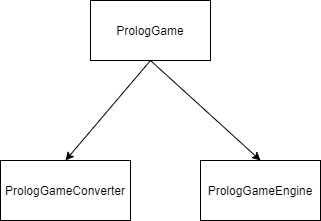
\includegraphics[scale=0.6]{prolog}
\end{center}
Di seguito vengono descritte le classi:
\begin{itemize}
    \item \textit{PrologGame}: espone tutte le funzionalità implementate attraverso tale linguaggio. Ogni qualvolta che si deve eseguire una funzionalità in Prolog, è necessario richiamare una funzione di questa classe corrispondente all’azione di Prolog.
    In particolare permette di creare le carte corredate da un valore, un seme e un colore per formare il deck di gioco, di eseguire la validazione di una combinazione di carte, che sia essa una scala, un tris o un poker e ne esegue l’ordinamento per seme e per valore.

    \item \textit{PrologEngine}: esegue effettivamente le azioni di Prolog.
    Si è deciso di realizzare un piccolo DSL che permettesse di facilitare l’utilizzo della libreria TuProlog e di aumentarne l’espressività del codice. Dopo aver caricato la specifica teoria, il \textit{PrologEngine} esegue le funzioni in grado di:
    \begin{itemize}
        \item risolvere un singolo obiettivo o più obiettivi;
        \item verificare se un obiettivo ha successo;
        \item se vi sono altre soluzioni dopo averne trovata almeno una;
        \item estrarre i valori dalle variabili, dopo l’esecuzione di un predicato, tramite la funzione \textit{bindingVars}.
    \end{itemize}

    \item \textit{PrologGameConverter}: questa classe espone funzioni in grado di formulare obiettivi nel giusto ‘formato’ in Prolog e di convertire il risultato ottenuto dal PrologEngine nel tipo corretto, a seconda dell’utilizzo. In particolare, grazie all’utilizzo dell’oggetto \textit{PrologUtils}, espone funzioni in grado di ‘pulire’ (da caratteri non conformi) il risultato del Prolog dopo averlo convertito in stringa. Questo è stato reso necessario poiché, quando si dava in input un obiettivo che conteneva una lista di tuple (ogni carta è una tupla che contiene nell’ordine valore, seme e colore), il risultato risultava essere ‘sporco’ da caratteri estranei rispetto al predicato dato in input.
    La classe permette infine di gestire la validazione di specifici casi, ad esempio  una combinazione che contiene uno o due assi. Essi, in una combinazione che forma una scala, possono essere posti uno prima del due e l’altro dopo del re, assumendo rispettivamente il valore di 1 o 14 a seconda della posizione inserita in una scala. La funzione \textit{OptionalValueAce} gestisce i casi appena descritti cambiando il valore dell’asso da 1 a 14.
\end{itemize}

\paragraph{Predicati}
Per ottenere le funzionalità descritte è stato creato il file rules.pl nella cartella delle risorse del modulo \textit{Core}.
\newline \newline
I predicati che permettono di creare le entità sono:
\begin{itemize}
    \item \textit{color}: specifica il tipo di colore di una carta;
    \item \textit{suit}: specifica il tipo di seme di una carta;
    \item \textit{card}: definisce l’entità carta composta da un valore, seme e colore.
\end{itemize}

I predicati utilizzati per la validazione delle combinazioni sono:
\begin{itemize}
    \item \textit{lengthList}: permette di determinare la lunghezza di una lista;
    \item \textit{sameNumber}: verifica se all’interno della lista le carte hanno tutti lo stesso valore;
    \item \textit{sameSuit}: verifica se all’interno della lista le carte hanno tutti lo stesso seme;
    \item \textit{differentSuit}: verifica se all’interno di una lista è presente più volte lo stesso seme.
    Tale predicato ne utilizza internamente un altro chiamato \textit{sameElementList} che mantiene memorizzato il seme della prima carta per poter confrontarlo con tutte le altre carte della lista;
    \item \textit{endSequence}: verifica la giusta terminazione di una scala che termina con un asso posto dopo il re.
    Questo significa che non è possibile continuare la scala aggiungendo un due e via di seguito;
    \item \textit{checkOrderByValue}: in caso di una scala verifica se le carte sono in ordine di valore;
    \item \textit{validationQuarter}: verifica se una combinazione è un tris o un poker.
    La funzionalità di questo predicato è ottenuta grazie alla composizione dei predicati precedentemente descritti, posti nel seguente ordine: \textit{lengthList}, \textit{sameNumber} e \textit{differentSuit};
    \item \textit{validationChain}: verifica se una combinazione è una scala.
    La funzionalità di questo predicato è ottenuta grazie alla composizione dei predicati precedentemente descritti, posti nel seguente ordine: \textit{lengthList}, \textit{sameSuit}, \textit{endSequence} e \textit{checkOrderByValue}.
\end{itemize}

I predicati utilizzati per l’ordinamento delle carte sono:
\begin{itemize}
    \item \textit{priority}: definisce la priorità dei semi.
    L’ordine utilizzato è: cuori, quadri, fiori e picche;
    \item \textit{quickSortSuit}: esegue l’ordinamento per seme.
    Internamente utilizza il predicato \textit{compareCard} per ordinare per valore tutte le carte dello stesso seme in base alla priorità;
    \item \textit{quickSortValue}: esegue l’ordinamento per valore.
\end{itemize}
Gli algoritmi di ordinamento quicksort per valore (o seme) a sua volta implementano il predicato \textit{partitionValue} (o \textit{partitionSuit}) che specifica la condizione necessario per ordinare.
\newline \newline
Descrivere le funzionalità più complesse come composizione di singoli predicati specifici ha permesso una maggiore leggibilità e manutenibilità del codice, in modo da poterli riutilizzare più volte all’interno della teoria.

\subsubsection{Game Interface}
\begin{center}
    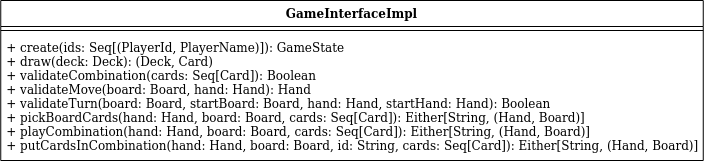
\includegraphics[width=\textwidth]{classi-Page-2}
\end{center}
Consiste in un insieme di funzioni utilizzabili dall’esterno del core per effettuare le normali operazioni che un giocatore reale farebbe durante una partita.
Queste operazioni comprendono:
\begin{itemize}
    \item Creare uno stato iniziale di una partita dato il numero e il nome dei players da aggiungerci;
    \item Pescare una carta da un mazzo;
    \item Validare una combinazione di carte;
    \item Validare una Hand e una Board, cioè una mossa effettuata da un giocatore. Validare una Hand significa controllare che non vi siano carte prese dal tavolo e non più riposte;
    \item Validare un turno intero, quindi confrontare una Hand e una Board attuale con la Hand e la Board di inizio turno;
    \item Prendere delle carte da una CardCombination in una Board;
    \item Giocare delle carte da una Hand in una Board in una CardCombination esistente;
    \item Giocare una nuova CardCombination da una Hand su una Board.
\end{itemize}
Il risultato dei vari metodi consiste in un oggetto complesso, un Either, che può contenere un valore piuttosto che un altro a seconda del risultato di un’altra funzione. Esso viene usato per poter gestire in modo consistente gli errori che eventualmente possono essere lanciati all’interno delle relative funzioni. Questo permette di evitare di lanciare delle eccezioni che non sono corrette in un approccio funzionale.

\subsection{Client}
\begin{center}
    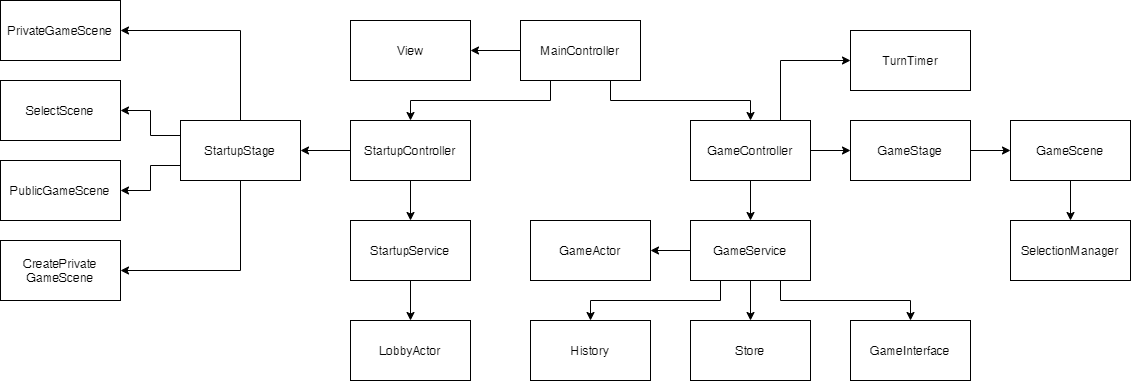
\includegraphics[width=\textwidth]{architetturaClient}
\end{center}

\subsubsection{MVC}
Per la parte client dell’applicazione si è scelto di utilizzare una architettura basata sul pattern MVC\@.
Questa ci ha consentito di tenere, anche all’interno del client, un buon livello di separazione tra le singole classi.
\newline
All’avvio dell’applicazione \textit{AppLauncher} avvia \textit{MainController}, che istanzia una istanza di View che fa da contenitore per entrambe le due parti di gioco (quella di avvio e quella di partita).
\textit{MainController} avvierà prima \textit{StartupController} per la parte di iscrizione alle lobby, e una volta ricevuto da quest’ultimo l'evento di creazione della partita, avvia il \textit{GameController}.
Ciascun controller setta nella view il proprio Stage e istanzia la classe Service, che nel MVC gioca il ruolo di model.
\begin{center}
    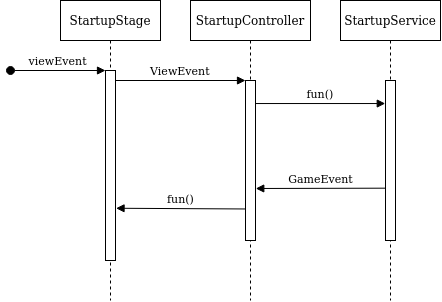
\includegraphics[scale=0.5]{messaggi_Startup_client}
\end{center}
Come si può notare dallo schema, il controller, per notificare eventi alla view, avendo creato il relativo \textit{Stage}, richiama i metodi che questo espone.
\newline
Allo stesso tempo, in creazione passa anche \textit{onViewEvent()}, una funzione che viene invocata dalla view ogni qualvolta debba notificare un evento al controller.
Questa funzione prende in input un oggetto di tipo case class/object che estende la sealed class \textit{ViewEvent}.\newline
Questa scelta di utilizzare da una parte l’interfaccia e dall’altra un metodo a callback è dovuta al fatto che logicamente, la view può notificare al controller qualsiasi tipo di evento, e sarà il controller a decidere quale di questi gestire; al contrario la view espone solamente le funzionalità che espone nella propria interfaccia.
\newline \newline
Simile è anche l’interazione tra \textit{Service} e \textit{Controller}. Il Controller avendo creato il Service ha il suo riferimento ed invoca i metodi che questo espone nella sua interfaccia. Allo stesso tempo passa in creazione il metodo \textit{notifyEvent()} che viene chiamato dal Service quando deve notificare un cambiamento di stato.

\subsubsection{View}
In entrambi gli stage \textit{Stage} vengono caricate le varie scene, ciascuna delle quali ha un interfaccia di metodi che possono essere chiamati dallo Stage che la contiene.
\newline \newline
Per velocizzare la creazione degli elementi di view più utilizzati, sono state creati degli object che contengono i factory methods per creare i relativi elementi:
\begin{itemize}
    \item \textit{ScalavelliButton}, factory per gli oggetti Button;
    \item \textit{ScalavelliLabel}, factory per gli oggetti Label;
    \item \textit{ScalavelliAlert}, factory per gli oggetti Alert;
    \item \textit{ScalavelliTextField}, factory per gli oggetti Button.
\end{itemize}
L’object \textit{CardUtils} è invece una utility che permette di ottenere il percorso dell’immagine raffigurante la carta da gioco a partire dall’entità \textit{Card}. \newline \newline
Si è scelto di gestire la visualizzazione degli alert e degli errori direttamente da \textit{Stage} in quanto questa operazione deve essere indipendente dalla scena in cui ci si trova.
Tutti i metodi che agiscono sugli elementi già renderizzati dalla view e gli aggiornamenti di stato hanno l’esigenza di agire sullo stesso thread di ScalaFX. Per poter ottenere questo risultato sono stati eseguiti all’interno della chiamata a \textit{Platform.runlater()}. \newline \newline
Le informazioni e la configurazione comune sia allo StartupStage che al GameStage sono contenute all’interno della classe \textit{BaseStage}.

\paragraph{Lobby}
\begin{center}
    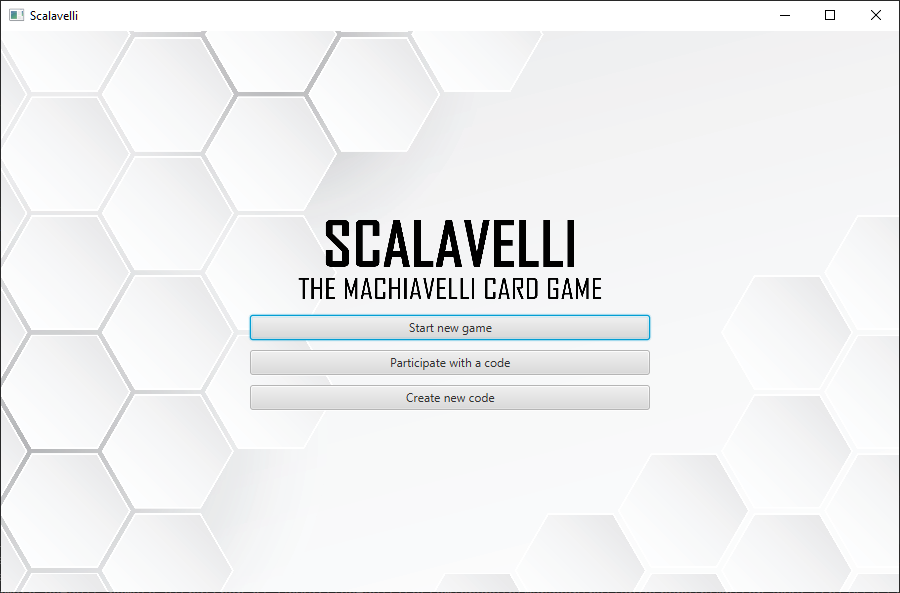
\includegraphics[scale=0.5]{home}
\end{center}
La parte di view si caratterizza di 4 scene che vengono caricate all’interno di \textit{StartupStage}. La scena principale permette di scegliere tra le 3 modalità di iscrizione a disposizione:
\begin{enumerate}
    \item Iscrizione ad una lobby pubblica, in base al numero di players selezionati;
    \item Iscrizione ad una lobby privata, inserendo un codice segreto:
    \item Creazione di una lobby privata, selezionando il numero di membri necessari per questa lobby.
\end{enumerate}
Alla selezione di una di queste modalità, viene caricata una nuova scena, alla quale viene passato un listener di tipo \textit{StartUpSceneListener} che tramite callback permette di reagire alle azione di \textit{submit()} e della pressione del tasto back.
\newline \newline
Tutte le scene estendono la classe astratta \textit{BaseStartupScene} che contiene la configurazione comune a tutte le scene. Questa classe è a sua volta estesa da \textit{BaseStartupFormScene}, la quale aggiunge i metodi comuni a tutte le scene in cui l’utente si iscrive ad una lobby, come ad esempio quelli per mostrare il messaggio di caricamento, per disabilitare i pulsanti e per ripulire gli input digitati.
\newline \newline
Ciascuna scena che estende \textit{BaseStartupFormScene} si compone di 3 parti:
\begin{itemize}
    \item \textit{StartupSceneTopBar}, che contiene il pulsante per tornare alla schermata precedente;
    \item \textit{StartupSceneBottomBar}, che contiene il pulsante di invio e la rotella di caricamento mentre si è in attesa della creazione di una partita;
    \item Un nodo centrale in cui è possibile l’inserimento dei dati (numero dei giocatori e username) o, nel caso della creazione di un codice segreto, la visualizzazione di quest’ultimo.
\end{itemize}

\begin{center}
    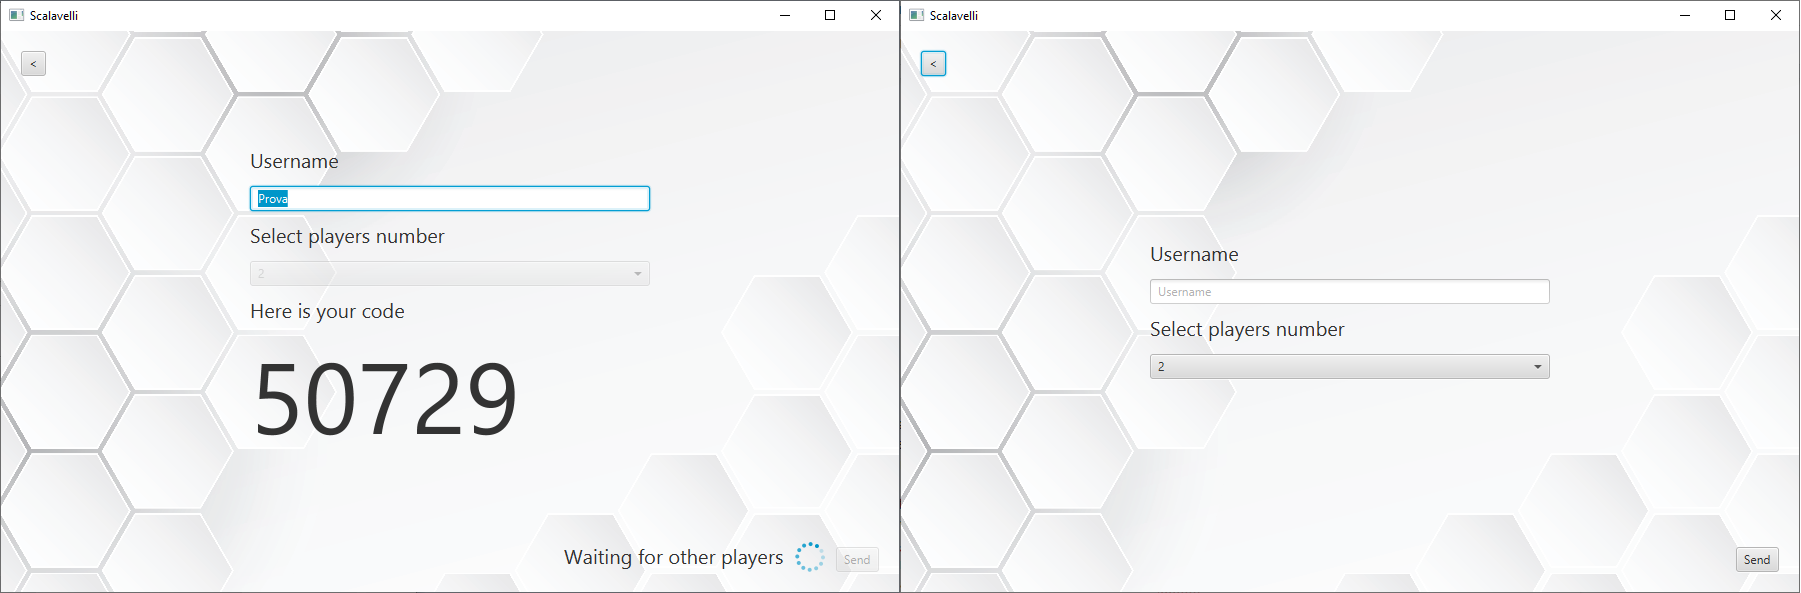
\includegraphics[scale=0.3]{create_join_lobby}
\end{center}

\paragraph{Game}
\begin{center}
    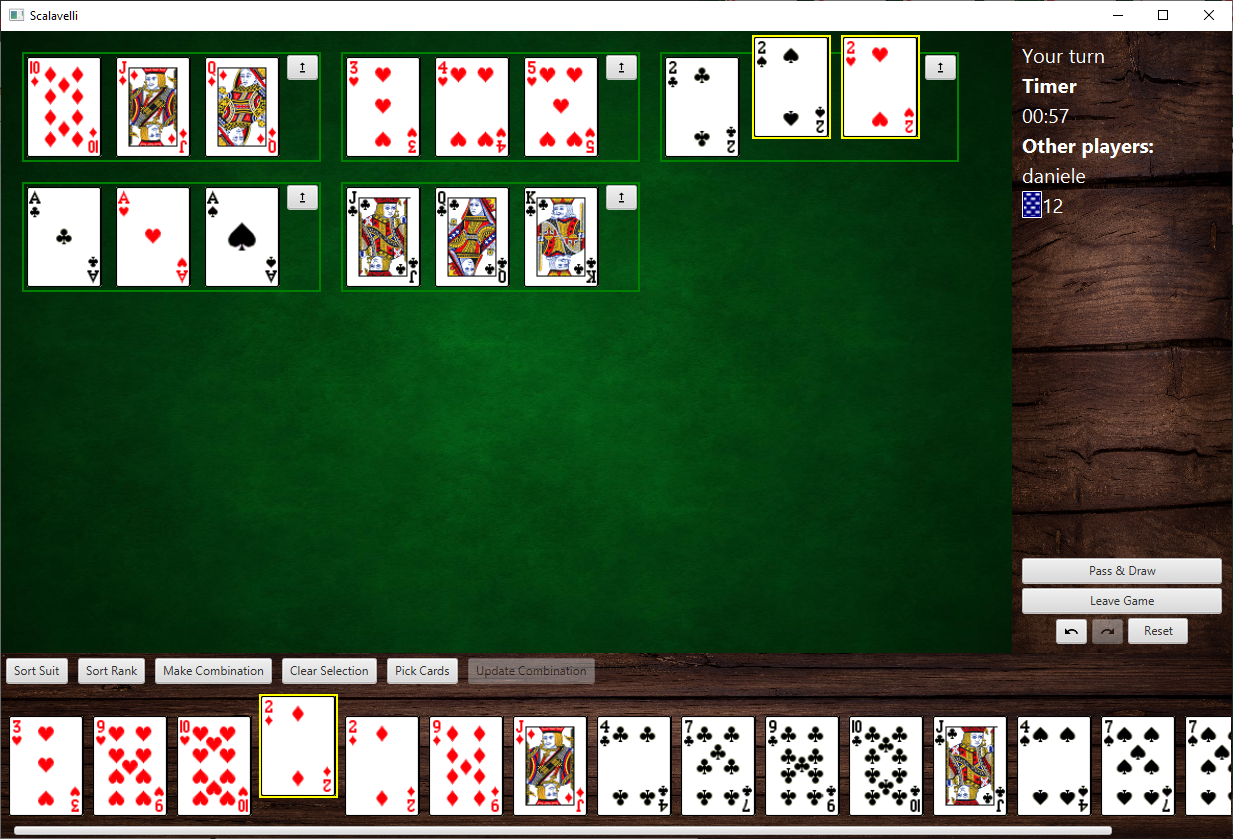
\includegraphics[scale=0.4]{game}
\end{center}
La view per la parte di Game si compone di una singola scena, GameScene, la quale si aggancia alla View attraverso GameStage.In questa schermata sono visualizzate tutte le informazioni di gioco e viene resa possibile l’interazione del giocatore con la partita. \newline
\begin{center}
    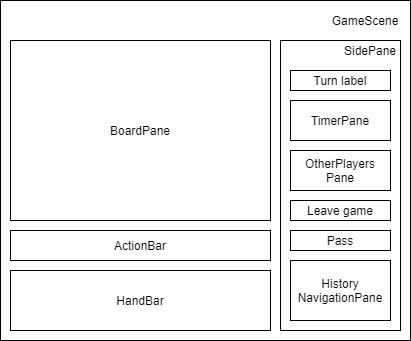
\includegraphics[scale=0.5]{viewPanes}
\end{center}
La view si compone di diversi Panes che sono stati implementati in classi distinte. Ciascun Pane ha anche la sua interfaccia che descrive i metodi che espone il pannello.
Ciascun pannello prende in input anche un listener con le callback che vengono istanziate all’interno della GameScene, nella quale vengono creati tutti i Panes.
\newline \newline
Ciascun Pane è stato pensato in modo da racchiudere poche funzionalità simili tra loro, in modo da avere un codice più leggibile e riutilizzabile:
\begin{itemize}
    \item \textit{BoardPane}: permette di visualizzare la board del gioco, permettendo all’utente di selezionare le singole carte, le combinazioni e di poter raccogliere le intere combinazioni dal tavolo;
    \item \textit{ActionBar}: contiene tutti i pulsanti tramite i quali l’utente può fare una giocata o riordinare la sua mano;
    \item \textit{SidePane} invece è il pannello laterale, e contiene a sua volta diversi pannelli:
    \begin{itemize}
        \item una label di informazione sul turno corrente;
        \item \textit{TimerPane}, dove viene mostrato il tempo a disposizione durante il turno del giocatore;
        \item \textit{OtherPlayersPane}, in cui vengono visualizzate il numero di carte che gli altri giocatori hanno in mano;
        \item \textit{HistoryNavigationPane} tramite il quale è possibile navigare la history e resettare il proprio turno;
        \item pulsanti per passare il turno e lasciare la partita.
    \end{itemize}
\end{itemize}
Ciascun \textit{Pane}, sul quale è possibile abilitare o disabilitare le azioni quando non è il turno del giocatore, estende il trait \textit{ActionGamePane}.
\newline
\begin{center}
    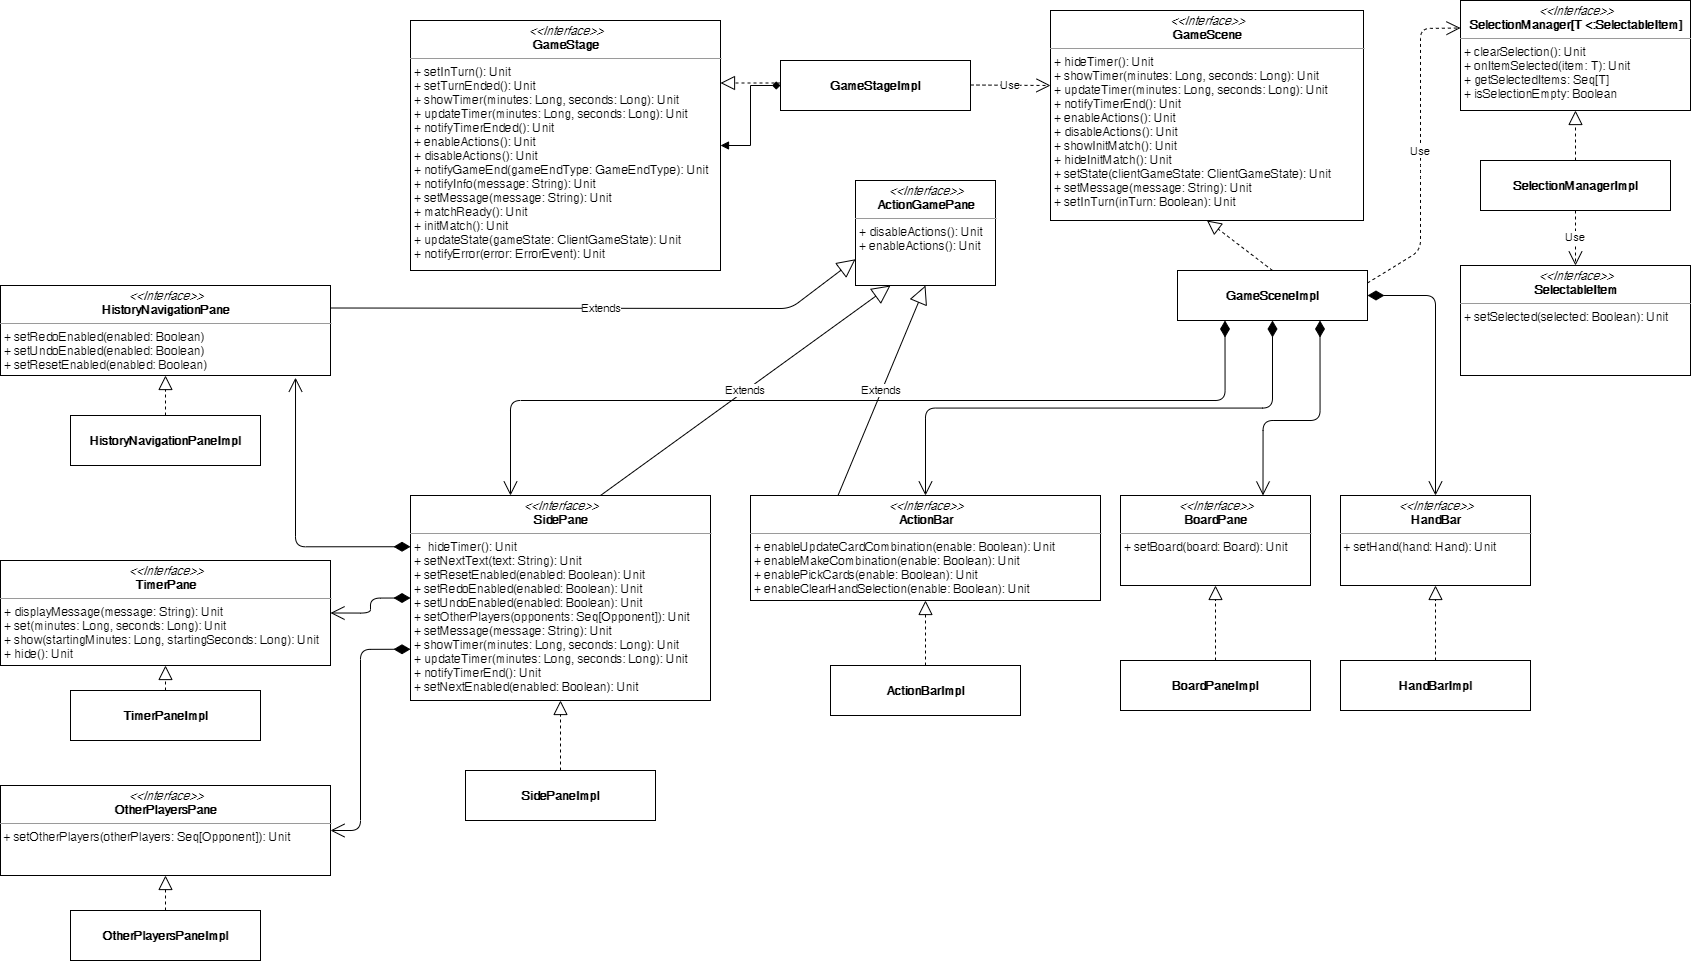
\includegraphics[scale=0.2]{gameViewArchitecture}
\end{center}
All’interno di \textit{GameScene}, attraverso più istanze della classe SelectionManager, si tiene traccia delle carte e delle combinazioni selezionate e deselezionate.\newline SelectionManager è generico in T, con T che estende SelectableItem, un trait che espone i metodi per settare un oggetto come selezionato o deselezionato.\newline Così facendo, SelectionManager avrà la sola responsabilità di tenere traccia degli elementi selezionati, mentre sarà l’elemento stesso ad implementare cosa avviene al momento della selezione, questo secondo il principio di singola responsabilità. \newline \newline
\textit{SelectionManager} prende in costruzione il parametro booleano \textit{allowOnlyOne} che indica se è possibile selezionare solamente un elemento per volta (deselezionando quindi quello precedente) o se al contrario, sia possibile selezionare più elementi. \newline Questa classe espone, oltre al metodo per selezionare o meno un elemento, i metodi per ottenere gli elementi selezionati e per pulire la selezione. \newline \newline
Le azioni che prevedono di avere accesso alle carte selezionate dalla mano o dalla board vengono gestite direttamente all’interno di GameScene, dove si ottengono le carte selezionate e vengono mandate al Controller. \newline \newline
GameStage espone tutti i metodi per mostrare messaggi di informazione, errore, terminazione della partita, aggiornamento del timer ma soprattutto, il metodo \textit{updateState()} che permette di aggiornare in continuazione lo stato della partita, sia durante il proprio turno, sia durante il turno degli altri giocatori.
\newline \newline
Questo metodo prende in input un oggetto di tipo \textit{ClientGameState} che oltre allo stato della board, della mano e degli altri giocatori, contiene anche le info sulla navigabilità della history (se è possibile fare undo/redo/reset) e sul fatto che sia già stata fatta o meno una azione dall’utente, così da poter aggiornare il testo del pulsante per il passaggio del turno.\newline Per togliere questa logica dalla parte di view, sarà comunque responsabilità del controller a controllare se l’utente potrà passare semplicemente o se invece quest’ultimo dovrà pescare una carta.
\subsubsection{Controller}
\paragraph{Lobby}
\textit{StarupController} avvia la view che permette all’utente di selezionare la modalità con cui partecipare ad una lobby e l’inserimento dei suoi dati. Una volta fatto questo, tramite l’interazione con \textit{StartupService} comunica al server la scelta dell’utente. \newline Da questo momento in poi l’utente resta in attesa di ricevere l’avvio del gioco da parte del Service, il quale comunica al Controller l’avvio del match.\newline
Per poter passare alla parte di Game avendo già il riferimento alla partita, a \textit{StartupController} è stato passato in costruzione la funzione \textit{startGame()} che viene invocata passando come parametro un oggetto di tipo \textit{GameMatchInformations} che contiene l’id dell’utente e il riferimento all’attore del match, il quale è stato costruito da \textit{StartupService}.
\paragraph{Game}
\begin{center}
    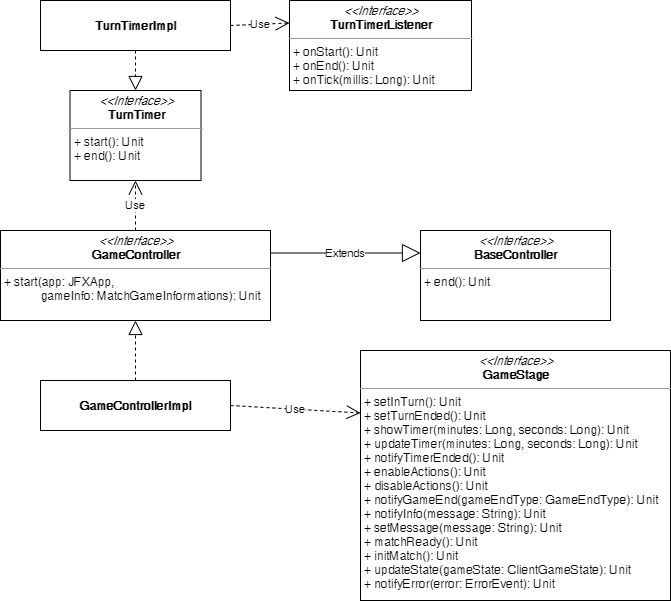
\includegraphics[scale=0.5]{gameController}
\end{center}
\textit{GameController} viene inizializzato direttamente da \textit{MainController}, il quale gli passa in costruzione anche la funzione da invocare per ricominciare una nuova partita.\newline \textit{GameController} istanzia e comunica con \textit{GameService}, invocandone i metodi esposti dall’interfaccia. In creazione invece passa la funzione \textit{notifyEvent()} che mappa in entrata gli eventi di tipo \textit{GameEvent}.\newline
Alla ricezione di questi chiama i metodi esposti dall’interfaccia \textit{GameStage}, aggiornando la schermata mostrata al giocatore. \newline \newline
Anche in questo caso, quando l’utente compie un'azione, viene generato un evento di tipo \textit{ViewGameEvent} e viene chiamata la funzione \textit{onViewEvent()} alla quale viene passato l’evento come parametro. Questo viene gestito da \textit{GameController} che sceglie quali metodi di \textit{GameService} chiamare.
\newline \newline Oltre a fare da collante tra Service e View, a \textit{GameController} è lasciata la responsabilità della gestione del timer durante il turno del giocatore. \newline Questo timer, per scelta a livello di design è stato lasciato solamente lato client, ed è implementato sfruttando le librerie Timer e TimerTask di java.utils. \newline \newline Espone tramite interfaccia i metodi \textit{start()} e \textit{stop()}, con i quali si avviano i due task che vengono eseguiti per ciascun turno. \newline Il primo task, chiamato tickTask, ha un periodo di 1000ms e permette di notificare un evento ogni secondo. Il secondo invece, chiamato endTask ha il compito di far scattare un evento allo scadere del tempo definito all’interno del file Constants.\newline Quando un utente inizia il proprio turno, il timer viene avviato, mentre sia quando scade, sia quando un utente passa prima del termine del turno, viene stoppato, azione con la quale si fa la \textit{cancel()} di entrambi i task e la \textit{purge()} del timer. \newline \newline
Al timer vengono passati in costruzione la durata prevista e un listener che contiene le callback che vengono triggerate dai vari task. Tra queste c’è la \textit{onStart()}, che viene chiamata all’avvio del timer, la \textit{onEnd()}, che viene chiamata allo scadere di endTask, e la onTick() che viene invece chiamata a ogni passaggio di tickTask. \newline \newline Il controller ha anche il compito di decidere se al passaggio di turno, l’utente dovrà pescare o passare semplicemente. Per farlo si affida all’ultimo aggiornamento di stato ricevuto, facendone una copia di volta in volta, e controlla se in questo l’utente doveva pescare oppure no.
\subsubsection{Model}
La parte di model del client è rappresentata dai trait StartupService e GameService con tutte le strutture a loro collegate. Rappresentano il punto in cui risiede tutta la business logic del client. Sono entrambi delle interfacce che espongono tutte le funzionalità rese disponibili dall’applicazione, su cui in controller si appoggiano per eseguire tutte le operazioni risultanti dalle azioni utente effettuate attraverso l’interazione con la view. \newline Permettono quindi di astrarre ai componenti utilizzatori le modalità con cui le varie azioni vengono risolte, ad esempio decidere se risolverle in locale o in remote contattando il server.
È solamente in questa parte del codice client che sono presenti riferimenti al framework akka. A differenza del server, il client non è stato modellato totalmente ad attori: questi sono stati utilizzati solo per la parte di comunicazione con il server tramite scambio di messaggi.
\paragraph{StartupService}
\begin{center}
    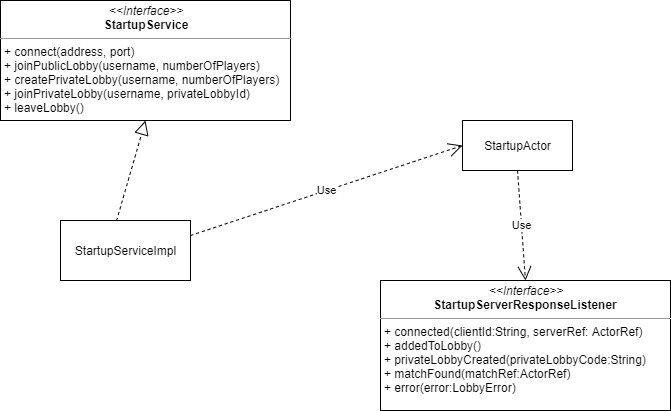
\includegraphics[scale=0.5]{server-startup-service}
\end{center}
È il componente che si occupa della gestione della lobby.
La sua funzione primaria, essendo la lobby gestita totalmente lato server, è quella di comunicare con quest’ultimo. \newline La connessione al server viene fatta tramite tramite il metodo \textit{actorSelection} messo a disposizione dall’unica istanza dell’oggetto \textit{ActorSystem} presente nell’object \textit{ActorSystemManager}, in caso di connessione avvenuta, si ottiene il riferimento all’attore remoto \textit{serverLobbyRef} responsabile per la gestione delle lobby, che viene utilizzato per l’invio dei successivi messaggi di richiesta di aggiunta alla lobby. \newline
I messaggi di risposta del server vengono invece ricevuti tramite l’attore \textit{StartupActor}, creato all’inizializzazione dell’oggetto sempre tramite l’istanza di \textit{ActorSystem}, il cui riferimento viene passato al server al momento della connessione.\newline Questo attore ha l’unica funzione di ricevere i messaggi inviati dal server e di redirezionarli tramite il trait \textit{StartupServerResponsesListener} che richiede in costruzione.\newline
La decisione di comunicare con il server su due vie separate è stata fatta per evitare duplicazione di messaggi: far fare tutto a StartupActor avrebbe richiesto l’invio di messaggi a quest’ultimo che a sua volta avrebbe dovuto inviarli al server.
I risultati delle varie operazioni vengono poi notificati al controller attraverso la funzione \textit{notifyEvent} richiesta in costruzione, a cui viene passato un oggetto di tipo \textit{GameStartupEvent}.\newline Il risultato della fase di lobby è l’oggetto \textit{GameMatchInformations}, che racchiude tutte le informazioni necessarie a poter avviare la partita lato client, come l'id del giocatore e la reference all'attore remoto del server.
\paragraph{GameService}
\begin{center}
    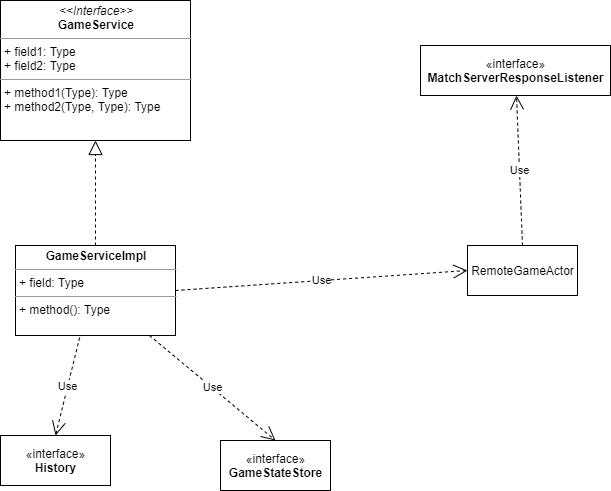
\includegraphics[scale=0.5]{server-game-service}
\end{center}
È il componente che si occupa di gestire lato client tutta la fase di gioco.
Come il componente descritto in precedenza per la fase di lobby, anche questo consiste in un’interfaccia che espone tutti i metodi corrispondenti alle funzionalità rese disponibili dal client di gioco.\newline La sua implementazione \textit{GameServiceImpl} è poi caratterizzata da diversi elementi, ciascuno dei quali gestisce una componente specifica del gioco.\newline Il riferimento all’attore server remoto \textit{serverActorRef} utilizzato per inviare messaggi al server. \textit{ClientGameActorRef}, il riferimento all’attore locale, responsabile di ricevere i messaggi inviati dal server, con una struttura analoga a quella descritta precedentemente per la lobby.
\newline GameStateStore utilizzato per mantenere lo stato locale della partita ed aggiornarlo a seguito delle azioni compiute dall’utente o dagli aggiornamenti ricevuti dal server. History, una struttura dati immutabile utilizzata per salvare lo storico degli stati risultanti dalle mosse eseguite dall’utente durante il turno. In seguito ad ogni mossa effettuata dal giocatore durante il turno, la History viene aggiornata e utilizzata per ripristinare lo stato delle versioni precedenti a seguito delle azioni di undo/redo.\newline \textit{GameInterface}, l’interfaccia core utilizzata per eseguire in locale le azioni di gioco effettuate durante il turno. \newline In costruzione riceve poi una funzione che utilizza per notificare al chiamante (in questo caso il controller) gli aggiornamenti di stato e gli altri eventi di sistema.
\newline
\newline
Di seguito la sequenza di operazioni che avvengono durante il turno di un giocatore quando quest’ultimo esegue una mossa:
\begin{itemize}
    \item Un chiamante invoca un metodo del \textit{GameService} corrispondente a un’azione di gioco;
    \item \textit{GameService} risolve l’azione per mezzo di \textit{GameInterface};
    \item Sulla base dell’output della funzione invocata su \textit{GameInterface} viene aggiornato lo stato locale di gioco tramite un metodo di \textit{GameStateStore};
    \item Il nuovo stato di gioco viene salvato sulla \textit{History};
    \item Il nuovo stato di gioco viene notificato al componente sottostante per mezzo della funzione notifyEvent ottenuta in costruzione.
\end{itemize}
Nel caso di una mossa eseguita in remoto la chiamata al \textit{GameInterface} è sostituita con un messaggio inviato al \textit{Server}, mentre manca l’aggiornamento della \textit{History} che viene utilizzata solamente durante la gestione locale del turno.
\subsection{Server}
È la componente che permette lo svolgersi del gioco in modalità multiplayer.Ogni sessione utente è possibile distinguerla in 2 fasi principali:
\begin{itemize}
    \item una fase di startup o lobby: in questa fase l’utente, una volta avviata l’applicazione, cerca di connettersi al server inviandogli i dati necessari per poter trovare una partita.
    Il server contemporaneamente rimane in attesa di connessioni dei client.
    Una volta connessi e ottenute le loro informazioni di gioco li inserisce all’interno della lobby, in attesa che si verifichino le condizioni necessarie affinché una partita possa essere generata.
    Al raggiungimento di tali condizioni, viene creata una partita, inserendo i giocatori che vengono rimossi dalla lobby.
    \item una fase di gioco: questa fase gestisce lo svolgersi della partita ed è ulteriormente suddivisa in 2 sotto fasi:
    \begin{itemize}
        \item Fase di inizializzazione, in cui i client ricevono un messaggio del fatto che la partita è stata trovata e ne danno conferma al server.
        Il server aspetta i messaggi da parte di tutti i client e una volta ricevuti, viene generato lo stato iniziale della partita, comunicato ai giocatori.Ora il gioco può iniziare.
        \item Fase di gioco, in cui il server si occupa di far proseguire il gioco, determinando il giocatore corrente, ricevendo le sue mosse, aggiornando lo stato in maniera ciclica, fino al verificarsi delle condizioni di terminazione del gioco.
        Il client si occupa di intercettare tutti le azioni effettuate dall’utente durante la partita, di comunicarle al server al termine del turno e di ricevere le varie informazioni sullo stato di avanzamento della partita.
    \end{itemize}
\end{itemize}

\subsubsection{Lobby}
\begin{center}
    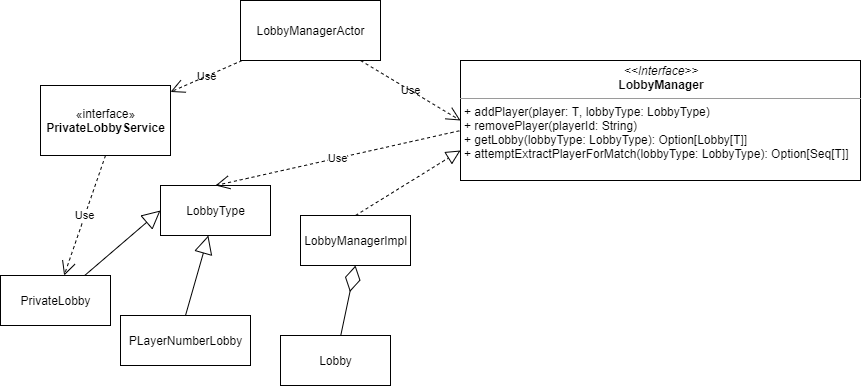
\includegraphics[width=\textwidth]{server-classi-lobby}
\end{center}
LobbyManagerActor è l’attore che si occupa di tutta la parte di gestione della fase di startup del gioco, è stato implementato estendendo il trait Actor di akka, rendendo quindi possibile la ricezioni di messaggi provenienti dai giocatori client.
Parte della logica di questo componente è stata poi portata fuori in altre strutture dati cercando di seguire il principio di Separation of Concerns.
Lobby è la struttura base che rappresenta una lista di giocatori accomunati dalle stesse preferenze riguardanti il numero di giocatori necessari per poter iniziare una partita.
LobbyManager è invece il componente che si occupa di mantenere i riferimenti a tutte le lobby create fino a quel momento, espone i metodi per inserire, rimuovere o estrarre i giocatori da una specifica lobby.
Per fare ciò mantiene una Lobby in corrispondenza di ogni LobbyType, che rappresenta l’informazione sulle caratteristiche di una lobby.

\paragraph{Modellazione delle lobby private}
La lobby privata presenta la caratteristica di una normale lobby di avere associato un valore corrispondente al numero di giocatori tale da poter essere estratti per formare un partita.Oltre a questo, ha un codice univoco per poterla identificare univocamente tra le tante.
PrivateLobbyService supporta la creazione di lobby private, generando un id univoco ogni volta che ne viene richiesta una nuova.

\paragraph{Interazione con il client}
\begin{center}
    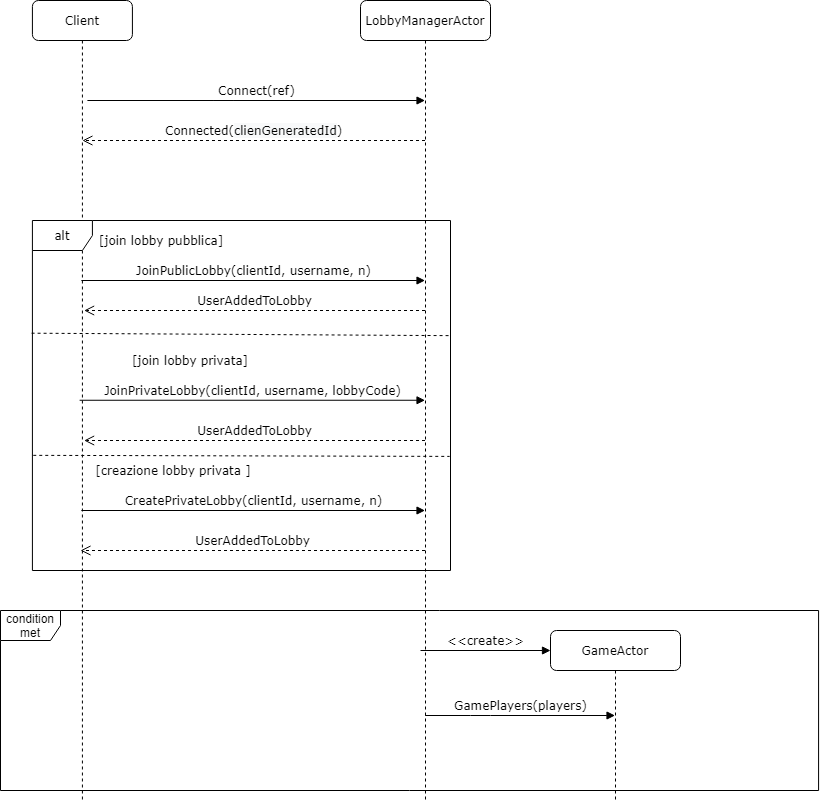
\includegraphics[width=\textwidth]{server-diagramma-attivita-lobby}
\end{center}
La sequenza di operazioni necessarie per poter entrare in una lobby e partecipare ad una partita è la seguente:
\begin{itemize}
    \item un client invia un messaggio Connect al server passandogli il riferimento all’attore client a cui quest’ultimo dovrà rispondere, a seguito del quale viene generato un id univoco che viene restituito al client;
    \item il client dopo aver scelto le preferenze di gioco, richiede al server di essere aggiunto ad una lobby (privata o pubblica) o di crearne una sua privata.
    Il server aggiunge il client alla lobby corrispondente rispondendo con un messaggio di avvenuta aggiunta.
    \item dopo aver aggiunto un giocatore ad una lobby, il server controlla se si sono verificate le condizioni per l’avvio di una nuova partita sulla lobby corrente tramite il metodo di LobbyManager attemptExtractPlayerForMatch che tenta di estrarre la lista di giocatori.
    In caso positivo i giocatori vengono rimossi dal sistema di lobby e viene creato un attore specifico per la partita GameMatchActor a cui vengono passati i loro riferimenti.Da quel momento in poi si occuperà di tutta la fase di gioco.
\end{itemize}

\subsubsection{Game}
\begin{center}
    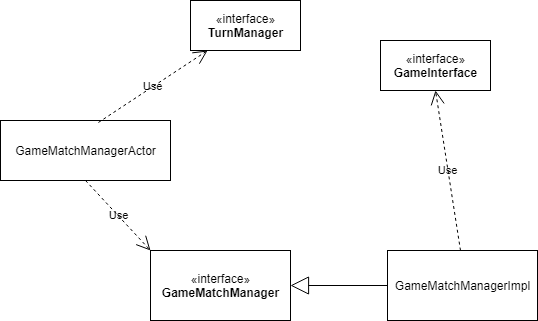
\includegraphics[width=\textwidth]{server-game-classes}
\end{center}
\textit{GameMatchActor} è l’attore server che si occupa della gestione di una partita, creato dall’attore Lobby descritto in precedenza.
Fa uso di due interfacce principali:
\begin{itemize}
    \item \textit{TurnManager} è la struttura che gestisce l'ordine del turno dei giocatori.Possiede la lista dei giocatori e la logica per determinare quello successivo a partire da quello corrente.
    \item \textit{GameHelper}, la cui implementazione è l’unica classe server che ha riferimento al core, espone i metodi necessari a creare lo stato iniziale della partita e a determinare lo stato successivo della partita sulla base dell’azione compiuta dal giocatore a fine turno.
\end{itemize}
Mantiene inoltre lo stato globale della partita, ad ogni suo aggiornamento lo trasmette a tutti giocatori connessi.
Per questioni di sicurezza, ad ogni giocatore non viene inviato lo stato globale ma uno stato parziale ricavato da esso con il metodo broadcastGameStateToPlayers, contenente le sole informazioni di interesse al giocatore (ad esempio l’informazione sul deck rimane solo al server, come anche la composizione delle mani degli avversari, che il giocatore corrente ovviamente non deve conoscere).

\paragraph{Comunicazione nella fase di inizializzazione della partita}
\begin{center}
    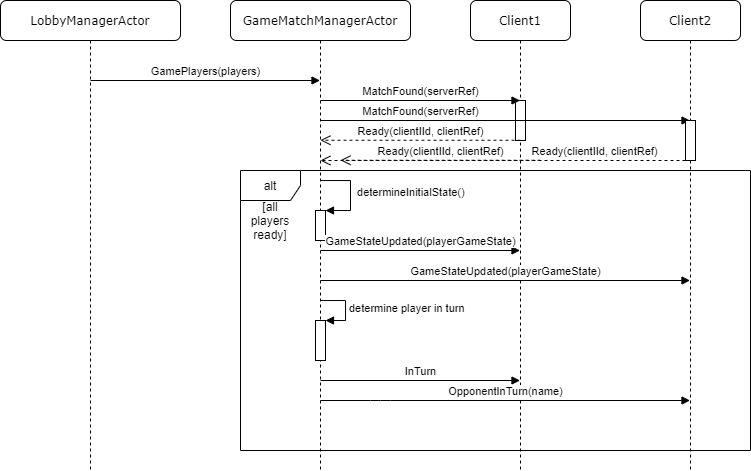
\includegraphics[width=\textwidth]{server-sequence-diagram-inizializzazione-gioco}
\end{center}
Una volta creato dall’attore lobby, l’attore responsabile della gestione della partita:
\begin{itemize}
    \item rimane in attesa di un messaggio di inizializzazione (GamePlayers) da parte di quest’ultimo, contenente le informazioni dei giocatori;
    \item notifica i giocatori che la partita è stata trovata tramite il messaggio MatchFound;
    \item rimane in attesa del loro messaggio di conferma Ready, contenente oltre all’id del giocatore il riferimento all’attore a cui inviare i successivi messaggi;
    \item ricevuti tutti i messaggi di conferma la partita viene inizializzata, viene generato lo stato iniziale ed inviato ai vari giocatori.Inoltre viene inviata una notifica al giocatore del turno corrente.
\end{itemize}

\paragraph{Comunicazione durante il turno di gioco}
\begin{center}
    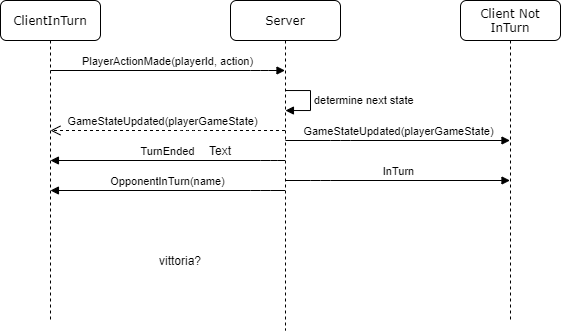
\includegraphics[width=\textwidth]{server-sequence-diagram-turno}
\end{center}
Una volta inizializzato il gioco e stabilito il giocatore corrente, il server rimane in attesa dell’azione di fino turno (le restanti azioni effettuate durante il turno sono gestite in locale come descritto in precedenza).
Dopodiché determina lo stato successivo sulla base dell’azione effettuata che può essere:
\begin{itemize}
    \item DrawCard: utente non effettua alcuna azione e decide di passare pescando una carta;
    \item PlayerMove(hand, board) : l’utente conclude il turno effettuando una o più mosse, con conseguente modifica della sua mano e del tavolo.
\end{itemize}
Determinato lo stato successivo, il server comunica la fine del turno facendo broadcast dello stato corrente a tutti i giocatori.Comunica la fine del turno al giocatore corrente e manda avanti la partita determinando il successivo.
\newline
Tutte queste operazioni verranno ripetute ciclicamente fino al verificarsi delle condizioni di vittoria, che comporta la notifica ai vari giocatori del termine della partita e la terminazione dell’attore server per la gestione della stessa.

\subsubsection{Fault Tolerance}
In entrambe le componenti del server (lobby e gioco) si è cercato di rilevare e gestire al meglio situazioni di errore come la disconnessione improvvisa dei client.
Per rilevare queste situazioni è stato utilizzata la funzionalità di supervisione e monitoraggio messa a disposizione da akka.\newline
Conoscendo il riferimento ad un attore è possibile ricevere gli eventi di terminazione, ricevendoli tramite il messaggio Terminated.\newline
L’attore lobby sfrutta questa funzionalità per rimuovere gli utenti terminati dalle code.
L’attore responsabile delle partita invece rileva la terminazione di uno dei giocatori, termina la partita stessa notificandola agli altri.

\subsection[Errori]{Gestione degli errori}
In tutte le componenti dell’applicazione si è cercato di evitare il più possibile la generazione di eccezioni qualora le funzioni avessero dovuto generare errori a causa dell’impossibilità di eseguire l’operazione richiesta.
Sono stati utilizzati dei meccanismi comuni sfruttando le funzionalità e le classi messe a disposizione dal linguaggio akka.
Option per evitare di avere valori null qualora la funzione non dovesse ritornare nulla.
Either per poter tornare un errore specifico nel caso in cui la funzione andasse in errore.
A questo scopo abbiamo creato delle classi di errore specifiche nei vari moduli.
Ad esempio nel metodo playCombination di GameInterface, in caso ci sia un errore nei parametri di input forniti, al posto di lanciare un’eccezione o di tornare un errore generico come Throwable, viene ritornato un oggetto della classe GameError, come CombinationNotValid.
\newpage


  \section{Implementazione}\label{sec:implementazione}
  \subsection{Matteo}
Per il progetto ho deciso di assumere il ruolo di Product Owner, mi sono occupato della coordinare il lavoro dei miei colleghi e di curare quanto possibile la bacheca trello, organizzando con l’aiuto degli altri le attività da svolgere in ogni sprint e cercando di tenere sempre sotto controllo lo stato dei lavori al fine di rispettare le scadenze programmate in principio.
A livello implementativo mi sono invece occupato della realizzazione della parte server in tutte le sue componenti.
Ho deciso di utilizzare il modello ad attori e un modello di comunicazione interamente basato su scambio di messaggi utilizzando il framework Akka in quanto l’ho ritenuto il modello ideale per modellare una situazione come quella di un gioco multiplayer, in cui ogni utente è caratterizzato da una fase “attiva” di gioco in cui esegue delle azioni, ma anche una “passiva” (nel caso specifico di Machiavelli quella del turno dell’avversario) in cui rimane silente ricevendo solo gli aggiornamenti del server riguardanti le mosse degli altri giocatori.
Ho lavorato anche sui file di configurazione di server e client per poter eseguire e testare il gioco in modalità multiplayer su una rete privata, e quindi non per forza su un unico computer.
Questi file di configurazione sono stati anche utile per poter personalizzare e visualizzare i log di akka, utili in certe fase dello sviluppo per poter identificare alcuni problemi durante il gioco reale, non venuti a galla in precedenza con i vari unit test realizzati.
L’altra componente di cui mi sono occupato è quella lato client della parte di Service sia dello lobby che di gioco, e strutture annesse:
\begin{itemize}
    \item Attori di lobby e di game per la comunicazione con il server.
    \item History, per la gestione dello storico delle mosse effettuate durante il turno del giocatore e poterci navigare avanti e indietro.
    \item GameStateStore, per la memorizzazione e l’aggiornamento dello stato locale della partita.
\end{itemize}
Ho poi contribuito alla realizzazione e modifica di alcuni elementi del core, aiutando anche a risolvere problemi sorti durante lo sviluppo.
In generale ho cercato sempre di curare la parte architetturale, facendo attenzione che le dipendenze tra classi e moduli dell’app venissero sempre rispettate.
Ho cercato anche di mantenermi il più possibile aderente allo stile di programmazione funzionale, preferendo sempre l’utilizzo di funzioni di libreria immutabili, promuovendo l’utilizzo di espressioni lambda e l’utilizzo di monadi come Either e Option.
Anche nelle classi realizzate ho cercato di seguire quando possibile il modello funzionale, prediligendo l’immutabilità, tranne in quei casi in cui a fronte di un’attenta analisi, ho optato per la creazione di strutture non totalmente funzionali con uso di side effect, come nei casi di classi caratterizzate dal fatto di mantenere uno stato locale aggiornato secondo delle funzioni esposte all’esterno, come il caso di LobbyManager lato server o GameStateStore sul client.

\subsection{Luca}
Per questo progetto ho assunto il ruolo di Committente, ruolo per il quale ho in primis cercato le regole e analizzato assieme a tutti gli altri elementi del gruppo le funzionalità che la nostra applicazione avrebbe dovuto supportare. \newline \newline Il lavorare sulla parte client, in particolar modo sulla view, oltre al fatto di essere il committente del progetto, mi ha permesso di tenere sempre sotto osservazione l’effettivo rispetto dei requisiti che ci eravamo prefissati, magari richiedendo anche agli altri membri del gruppo il supporto di una funzionalità che era sfuggita durante l’implementazione degli altri moduli.
\subsubsection{Sviluppo Client - View e Controller}
Durante lo sviluppo, invece, ho lavorato sulla parte client dell’applicazione, e dopo aver deciso di adottare il pattern MVC, ho lavorato specialmente sulle parti di View e Controller.\newline \newline In un primo momento ho valutato attentamente l’utilizzo della libreria ScalaFX, per vedere se avesse potuto portare delle difficoltà durante lo sviluppo per via di possibili funzionalità mancanti, le quali però non sono state evidenziate. \newline \newline Nello sviluppo ho sempre cercato di separare logicamente le funzionalità, i componenti della view, le parti di gioco in modo da permettere di avere una struttura modulare e ottenere delle classi più leggibili. A tal proposito ho spesso utilizzato i companion object per contenere la parte di implementazione ed utilizzare trait e classi astratte per esporre le funzionalità messe a disposizione dai vari elementi. Trait e classi astratte sono state utili anche per descrivere funzionalità e scrivere pezzi di codice comuni a più elementi di view. \newline \newline Anche per la creazione di pulsanti, labels, alerts e textFields ho deciso di utilizzare degli oggetti che contengono diversi metodi apply() a seconda di come si vuole creare quell’ elemento, e durante la scrittura del codice, la cosa si è rivelata molto utile.\newline \newline Sia per la creazione di TurnTimer che di SelectionManager, ho cercato di rendere le classi il più riutilizzabili possibile, nel primo caso avvalendomi delle callback per reagire agli eventi generati dai TimerTask, nel secondo creando una classe generica, che permetta di selezionare oggetti che implementano il trait SelectableItem, rendendolo utilizzabile anche in altri contesti.
\newline \newline Infine, assieme a Lorenzo e Matteo abbiamo lavorato ad un refactoring della gestione degli errori che, avendo suddiviso il progetto in più moduli distinti, potevano provenire da diverse parti. I testi degli errori, di informazione, così come tutte le label, sono stati gestiti solamente lato view, così da poterli in futuro modificare, magari aggiungendo il supporto multilingua.
\subsubsection{Interazioni nel MVC}
Sempre assieme a Matteo, il quale ha lavorato sulla parte di Model che interagisce con il Controller, ho valutato attentamente in quali casi fosse opportuno esporre una interfaccia di metodi e in quali passare una funzione con un evento come parametro. La scelta è ricaduta sul primo approccio per la comunicazione Controller-View e Controller-Model, mentre invece si è scelto il secondo per quella View-Controller e Model-Controller, in quanto View e Model generano comunque eventi e deve essere il controller a decidere quali gestire ed in che modo. Così facendo, è stato possibile aggiungere funzionalità alla View e al Model semplicemente dichiarando il nuovo tipo di evento, che sarebbe poi stato gestito alla necessità.\newline \newline Durante lo sviluppo ho poi fatto lavorato su GameService e History per riuscire ad ottenere le informazioni sulla possibilità di navigare la History da parte dell’utente. A tal proposito, assieme a Matteo si è deciso di creare l’oggetto ClientGameState che racchiudesse tutte le informazioni necessarie all’aggiornamento dello stato.
\subsection{Lorenzo}
Durante lo sviluppo del progetto ho cercato di mantenermi il più possibile consono allo stile della programmazione funzionale, cercando di mantenere uno stato immutabile nei punti in cui fosse necessario. \newline \newline Mi sono occupato principalmente della parte core del progetto: lavorando sulle entità che lo compongono e su tutta la logica correlata alla gestione delle regole necessarie per poter implementare il gioco. Quest’ultima parte è stata realizzata integrando Prolog con Scala.
\subsubsection{Entità - Core}
Assieme a Daniele ho definito e implementato le entità base per l’interazione tra esse e altri componenti del progetto.\newline Negli Sprint 3 e 4, ho revisionato questa parte per ottimizzare il codice.
\subsubsection{Prolog - Core}
La creazione delle entità e gestione delle regole è stata realizzata tramite il linguaggio Prolog.
In particolare ho creato il file rules.pl in cui ho definito tutte le regole di validazione che il gioco ammette (tris, poker e scale), ho realizzato l’ordinamento delle carte nella mano di un giocatore per seme e per valore e ho creato le entità di base del gioco.
Ho implementato tutta la parte in scala di gestione al prolog utilizzando la libreria TuProlog.
In quest'ultimo caso è stato necessario definire la classe \textit{PrologGameEngine} in grado di risolvere i vari goals dati in input ed ottenere i rispettivi risultati.
Ho definito la classe \textit{PrologGameConverter} che converte i risultati ottenuti da prolog in un formato conforme alle entità del progetto.
Quest’ultima classe non è stata banale implementarla poiché ho riscontrato alcuni errori della libreria TuProlog.
Questo accadeva quando il predicato specificato per risolvere un goal conteneva una lista di tuple.
Per questo motivo ho creato un oggetto ad-hoc, \textit{PrologUtils}, in grado di poter definire delle funzioni che permettevano di ‘pulire’ il risultato ottenuto con specifici caratteri per poterlo convertire nel formato richiesto (ad esempio una carta).
Infine ho aiutato gli altri membri nella realizzazione di alcuni task.
\subsection{Daniele}
\subsubsection{Continuous Integration}
Mi sono occupato di configurare opportunamente l'ambiente di CI scelto in modo da poter verificare la correttezza di ogni singola build, compilando ad ogni push su ogni branch e pull request.
Inoltre, documentandomi online, ho trovato molto utile anche il sito \textit{Codecov.io}, che si occupa di mantenere delle statistiche sulla copertura dei test sul progetto.
Per il rilascio della Relazione e Scaladoc ad ogni rilascio sul branch di dev ho scelto \textit{Github Pages} in modo da renderlo disponibile per tutti.
Per il rilascio dei pacchetti eseguibili degli applicativi server e client ad ogni push etichettata sul master ho scelto sempre \textit{Github Releases}.
Questa parte ha richiesto molto lavoro ancora prima di iniziare a sviluppare, ma successivamente tutto il team ne ha tratto beneficio.
In corso d'opera, si e trattato solamente di adattare mano a mano la configurazione già esistente alle crescenti esigenze del progetto (sopratutto in quanto a riduzione dei tempi di compilazione).
\subsubsection{Build automation}
Mi sono occupato inoltre degli script necessari per eseguire agilmente una compilazione di tutto il progetto o di parte di esso in base alle esigenze.
Tutto il progetto è stato incapsulato in moduli logicamente separati, seppur talvolta con dipendenze gli uni dagli altri.
Questo ha permesso tante volte di ridurre tempi morti, compilando o testando solamente parti del progetto.
\subsubsection{Core}
Assieme a Lorenzo mi sono occupato dello sviluppo delle entità base del progetto e di tutti quegli elementi di gioco che riguardavano le regole del gioco e le interazioni tra di esse.
Ho speso tanto tempo nel ottimizzare il codice e di slegarmi dallo schema mentale della programmazione ad oggetti che ho utilizzato fino a prima dell'inizio del progetto.
Ancora adesso penso di non essere riuscito appieno nell'impresa, dato che comunque anche al lavoro sono costretto ad usare comunque l'altro approccio.
\newpage


  \section{Retrospettiva}\label{sec:retrospettiva}
  \subsection{Organizzazione del processo di sviluppo}
Il processo di sviluppo è stato suddiviso in un primo sprint iniziale per confrontarsi sul design architetturale da adottare e discutere delle interazioni che i vari componenti dovevano avere.
In questo sprint abbiamo poi definito i quattro successivi di sviluppo del progetto.
Ogni sprint (eccetto quello iniziale) ha avuto mediamente una durata di circa 1,5/2 settimane.

\subsubsection{Preparazione iniziale}
Durante questo fase ci siamo incontrati più volte per definire l’architettura e i requisiti base che il nostro progetto doveva soddisfare.
Inoltre abbiamo individuato i componenti di gioco e le loro interazioni.
In questo modo abbiamo avuto l'opportunità di confrontarci e discutere per una migliore organizzazione dei successivi sprint.
Abbiamo inoltre configurato l’ambiente di sviluppo e assegnatoci i rispettivi compiti in base all’interesse di ognuno.
Tutta questa fase è stata completamente da remoto con lunghe chiamate su Microsoft Teams, tranne per l’ultima riunione in cui siamo riusciti a vederci tutti insieme.

\subsubsection{Sprint 1}
Questo sprint consisteva nel sviluppare le seguenti funzionalità:
\begin{itemize}
    \item Visualizzazione di una view di base della lobby in cui l’utente può inserire un username e il numero di giocatori con cui vuole partecipare.
    \item Per la parte server, creazione della lobby e gestione degli utenti in coda fino al raggiungimento necessario dei numeri di giocatori.
    \item Per il core, modellazione delle entità di gioco sia in Scala che in Prolog: colore, seme, valore, carte e le regole di validazione.
\end{itemize}
In questa fase abbiamo notato che il carico di lavoro per il facimento del Core e del Prolog è stato maggiore rispetto agli altri, dato che su di essi si sarebbe basato molto del lavoro del successivo sprint, causando una maggiore pressione nei due membri del team a cui è stato assegnato questo compito.

\subsubsection{Sprint 2}
Questo sprint consisteva nel sviluppare le seguenti funzionalità:
\begin{itemize}
    \item Creazione della struttura del client, collegamento del client con server durante la fase di registrazione ad una lobby.
    \item Inizio gioco: collegamento della lobby con lo stato iniziale della partita.
    \item View di gioco con la visualizzazione del tavolo e delle carte in mano ad un giocatore.
    \item Definizione dell’interfaccia core per la gestione del gioco.
    \item Arricchimento la libreria prolog con l’aggiunta dell’ordinamento delle carte per seme e per valore che fino a quel momento erano state implementate in scala.
\end{itemize}

\subsubsection{Sprint 3}
L’obiettivo di questo sprint era quello di collegare le singole parti sviluppate in modo da ottenere un collegamento tra client-core-server e view visualizzando le funzionalità delle partita.
Abbiamo terminato tutta l’implementazione del Core con qualche piccolo aggiustamento.
Da questo sprint in poi sono iniziati ad essere rilevati tanti problemi con la validazione delle combinazioni in Prolog, causati dalla molteplice valenza del valore Asso (come primo e ultimo valore di una scala e possibilità di essere presente in due copie).
\newline
Questo è stato lo sprint più importante di tutto il processo di sviluppo poiché sono stati completati molti task alla gestione del gioco.
Inoltre, abbiamo notato il problema inverso rispetto al primo sprint: il carico di lavoro sul Server e sul Client è stato maggiore che sul resto.
Tuttavia in questo caso è stato possibile per i due membri restanti aiutare gli altri nella realizzazione dei loro task.

\subsubsection{Sprint 4}
Nell’ultimo sprint ci siamo occupati di risolvere alcuni problemi legati al server come la disconnessione improvvisa da parte di un utente o l’abbandono della partita.
Inoltre, lato client, abbiamo implementato la gestione del tempo che ogni giocatore ha a disposizione per completare il turno.
In questa fase tutti i membri del team hanno contribuito a risolvere i bug e rifattorizzare il codice presente.

\subsection{Sviluppi futuri}
Di sicuro come prossimi sviluppi potrebbero essere affrontati tutti i punti opzionali che non siamo riusciti a svolgere entro il tempo del progetto, quali:
\begin{itemize}
    \item Funzionalità che suggerisca all'utente una possibile mossa da fare nel proprio turno.
    \item Semplice AI contro cui giocare in locale.
    \item Possibilità di personalizzare alcune caratteristiche di questo gioco.
\end{itemize}
Al di fuori di essi, principalmente si è pensato a:
\begin{itemize}
    \item modificare il server per poterlo installare su di un container da mettere su una macchina remoto raggiungibile da remoto in modo da poter estendere i possibili utenti utilizzatori del gioco, per creare partite più avvincenti ed un’esperienza d’uso più completa.
    \item creare una base dati per la memorizzazione dei risultati delle partite e degli utenti in modo da generare periodicamente una classifica dei migliori giocatori.
    \item migliorare la funzionalità di generazione di partite private per arrivare a creare dei veri e propri tornei.
    Gli utenti, inseriti dentro a delle maxi lobby private, all’avvio del turno di un torneo, verrebbero accoppiati ad altri giocatori in base ai risultati delle partite precedenti.
    Gli utenti tornerebbero nella stessa maxi lobby al termine del turno per poter di nuovo essere accoppiati.
    Regole di gestione del torneo ulteriori, come ad esempio i gironi all’italiana o i punti della classifica potrebbero essere scelte direttamente dai gestori del torneo.
\end{itemize}

\subsection{Commenti finali}

\end{document}